% !TeX root = ../ise-lab-ske.tex
\begin{figure}
    \centering

    \begin{tabular}{c|ccc}
        Predictor & \multicolumn{3}{c}{Extractor} \\
        \hline\hline
        & \real{} & \trepan{} & \cart{} \\
        \subfloat[5-NN.]{
            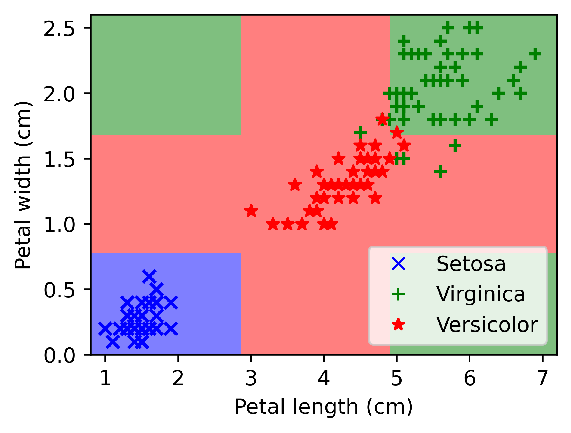
\includegraphics[width=0.20\linewidth]{img/CLA/bb-knn.pdf}
            \label{fig:bb-knn}
        } &
        \subfloat[]{
            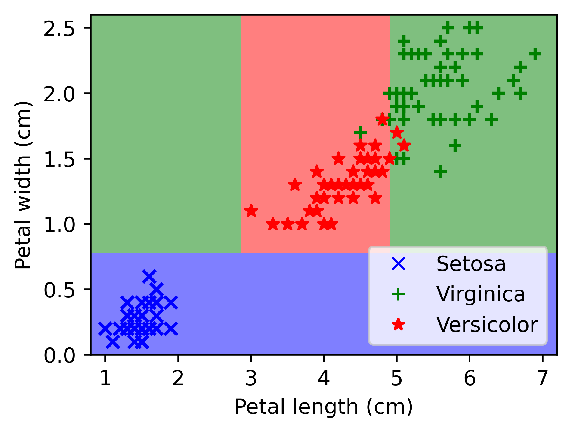
\includegraphics[width=0.20\linewidth]{img/CLA/real-knn.pdf}
            \label{fig:real-knn}
        } &
        \subfloat[]{
            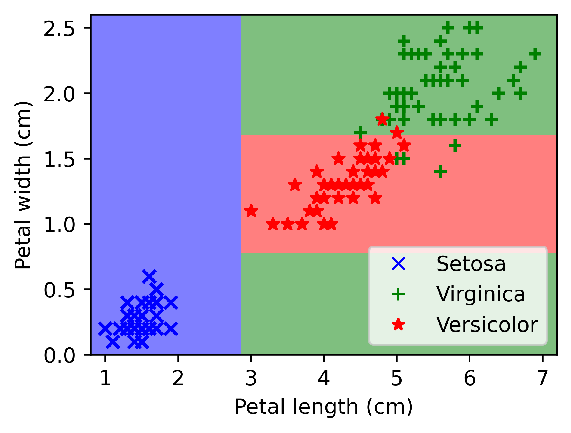
\includegraphics[width=0.20\linewidth]{img/CLA/trepan-knn.pdf}
            \label{fig:trepan-knn}
        } &
        \subfloat[]{
            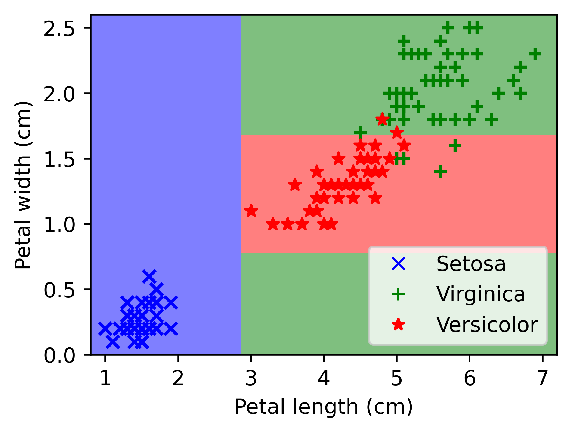
\includegraphics[width=0.20\linewidth]{img/CLA/cart-knn.pdf}
            \label{fig:cart-knn}
        } 
        \\
        \subfloat[MLP.]{
            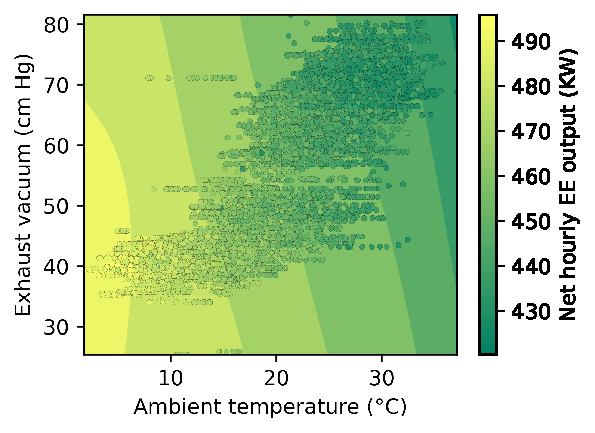
\includegraphics[width=0.20\linewidth]{img/CLA/bb-mlp.pdf}
            \label{fig:bb-mlp-cla}
        } &
        \subfloat[]{
            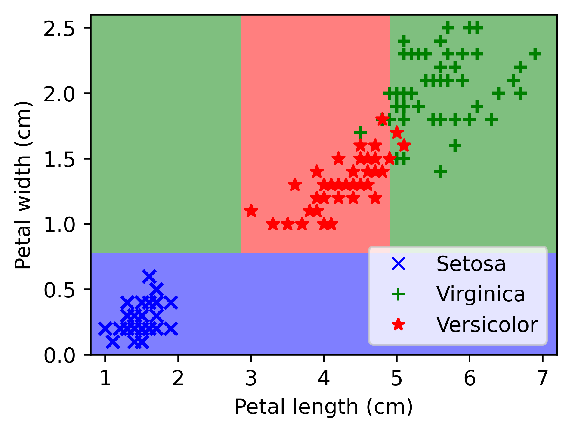
\includegraphics[width=0.20\linewidth]{img/CLA/real-mlp.pdf}
            \label{fig:real-mlp}
        } &
        \subfloat[]{
            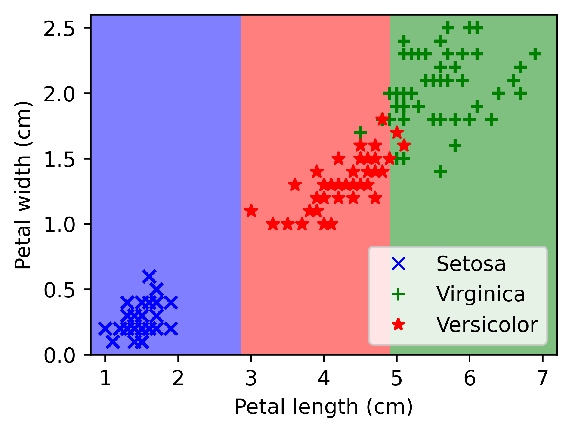
\includegraphics[width=0.20\linewidth]{img/CLA/trepan-mlp.pdf}
            \label{fig:trepan-mlp}
        } &
        \subfloat[]{
            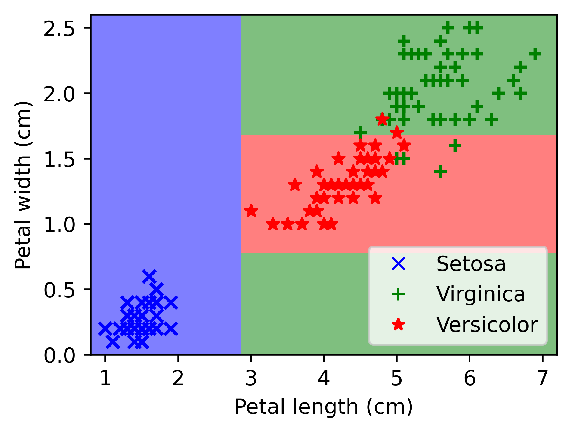
\includegraphics[width=0.20\linewidth]{img/CLA/cart-mlp.pdf}
            \label{fig:cart-mlp-cla}
        } 			
    \end{tabular}
\end{figure}